\documentclass[12pt]{extarticle}
\usepackage[utf8]{inputenc}
\usepackage{cite}
\usepackage[headheight=20pt,headsep=0pt]{geometry}
\usepackage{graphicx}
\usepackage{wrapfig}
\usepackage{hyperref}
\usepackage{xcolor}
\usepackage{IEEEtrantools}
\graphicspath{ {./images/} }


\title{Project Proposal \\
Natural Language Processing with Disaster Tweets
}
\author{Sina Abbasi}
\date{Feb. 2022}

\begin{document}
\maketitle
% \leftskip=-0.5in
% \rightskip=-0.5in


\section*{Motivation}

\begin{wrapfigure}{r}{0.4\textwidth}
    \begin{center}
    % \centering
    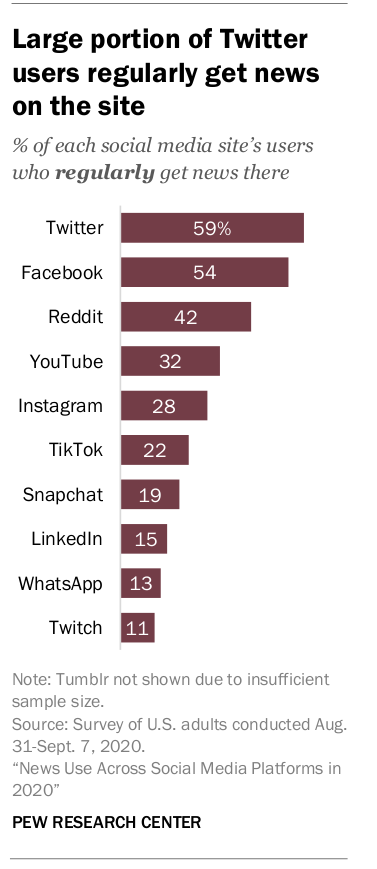
\includegraphics[width=0.3\textwidth,height=0.6\textwidth]{twitterfig1.png}
    \end{center}
    \caption{Percentage of users that get their news from that social media.}
    \label{fig:twitter}
\end{wrapfigure}

Nowadays, thanks to smartphones and easy access to internet across the world the free social media applications are one of the best places to get the breaking news instantly. Especially after COVID-19 hit, news consumption from social medias rapidly increased where based on Pew Research Center survey conducted 31 August - 7 September 2020, about half of US adults (53\%) get their news "often" or "sometimes" from social media \cite{shearer2021news}. Moreover, for example, about half of Twitter's users get their news from there as you can see in Fig. \ref{fig:twitter} \cite{shearer2021news}. Moreover, people use Twitter to report emergency news that are seeing them in real-time. Therefore, many companies and news agencies are interested to monitor the Twitter to get real-time and breaking news. More importantly, organizations such as disaster relief organization want to know the news about disasters as soon as possible. This monitoring can not be done by humans because we are dealing with on average 6000 tweets per second.\\

Pragmatically monitoring Twitter by just analyzing the words in each sentence separately is not a promising approach. For example, the author of a tweet said: "On plus side LOOK AT THE SKY LAST NIGHT IT WAS ABLAZE" \cite{tw}; the word "ABLAZE" is used not in actual meaning but metaphorically.\\


\section*{Project details}

In this project we are going to build a deep learning model that can classify which tweets are pointing a real disaster or not. Obviously, since we will work on text data, this task will be a Natural Language Processing (NLP) task. This challenge is a classification task and the sequential model (not trained model) can be used in other classification tasks in different domains, i.e. stock market predication based on tweets or news, sentiment classification for reviews of an online market like amazon, spam news classification and etc.\\

The input of the task will be text and the binary output should determine that weather the text describes an real disaster or not. The evaluation will be based on F1 score between predicted and expected answer and F1 is calculated as follow: 
\begin{IEEEeqnarray}{rCl}
    \label{eq:f1}
    F1=2\times \frac{precision\times recall}{precision+recall},
\end{IEEEeqnarray}
where
\begin{IEEEeqnarray}{rCl}
    \label{eq:precision}
    precision=\frac{TP}{TP+FP},
\end{IEEEeqnarray}
\begin{IEEEeqnarray}{rCl}
    \label{eq:recall}
    recall=\frac{TP}{TP+FN},
\end{IEEEeqnarray}
TP, FP and FN stands for true positive, false positive and false negative, respectively. $F1 = 1$ is the best value that means perfect precision and recall and $F1=0$ is the worst.
\\

\section*{Data set}

In Fig. \ref{fig:dataSamples}, you can see data set includes five columns where \\
\texttt{keyword}: a particular keyword from the tweet (may be blank)\\
\texttt{location}: the location the tweet was sent from (may be blank)\\
\texttt{text}: the text of the tweet\\
\texttt{target}: this denotes whether a tweet is about a real disaster (1) or not (0).\\
Train data has about 7.5k sample rows, and target values has fair distribution as you can see in Fig. \ref{fig:targetdist}.\\

\begin{figure}[!t]
\centering
%\includegraphics[scale=0.4]{img/figure1.eps}
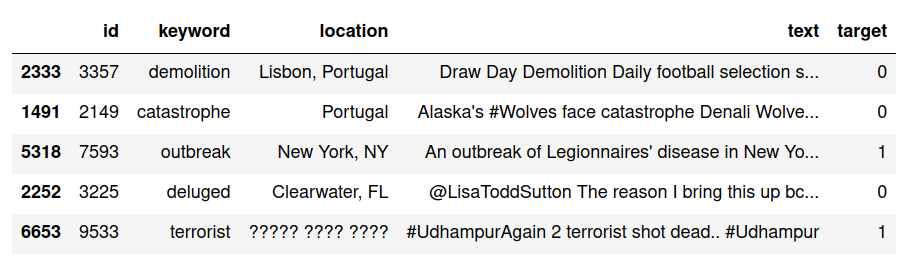
\includegraphics[width=1\textwidth]{images/dataSamples.png}
\caption{Data samples.}
\label{fig:dataSamples}
\end{figure}

\begin{figure}[!t]
\centering
%\includegraphics[scale=0.4]{img/figure1.eps}
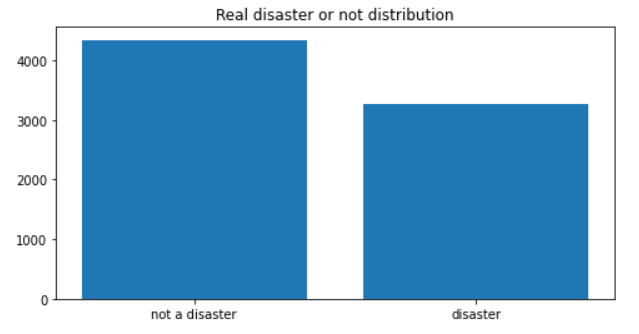
\includegraphics[width=0.8\textwidth]{images/distribution.png}
\caption{Distribution of target values.}
\label{fig:targetdist}
\end{figure}


\section*{Competition details}

The task is an active kaggle competition with currently 830 competitors that you can find it \href{https://www.kaggle.com/c/nlp-getting-started/}{\textcolor{blue}{\textit{here}}}. Best score is 1.0 (perfect score) and top 50 scores vary between 0.84 to 1.0.\\

\section*{Related works}
 
 Authors in \cite{sit2019identifying} works on similar data sets but the tweets related to hurricane. They get the data from Twitter and aiming to first classify and then analyse disaster-related tweets. In their binary classification phase, classification methods: LSTM, CNN, SVM, Logistic Regression and Ridge are performed and based on their evaluation Long Short-Term Memory (LSTM) get better fit to sequential order of textual data.
 
Looking through the top solutions in Kaggle website where they used LSTM structure to solve this task, we found and run a notebook which gave us 0.81 F1 score. This is a decent score for a NLP task. However, based on new viral method published by google researchers at 2018 called "BERT: Pre-training of Deep Bidirectional Transformers for Language Understanding" which has already 34000 citation, the BERT can learn better contextual text \cite{devlin2018bert}. Therefore, we are going to use this transformer for our task and try to get better F1 performance than LSTM.


 
\bibliographystyle{IEEEtran} 
\bibliography{refs}
\end{document}
